
\documentclass{dissertation}
%\documentclass[print]{dissertation}
%\documentclass[print,draft]{dissertation}

\makeatletter
\@ifundefined{widering}{}{%
	\let\widering\relax
}
\makeatother

\AtBeginDocument{%
	\DeclareSymbolFont{operators}{OT1}{ntxtlf}{m}{n}
	\SetSymbolFont{operators}{bold}{OT1}{ntxtlf}{b}{n}
}
\usepackage{bbm}
\newcommand{\1}{\mathbbm{1}}
\usepackage{bm}

\usepackage{setspace}
\onehalfspacing

%Some definitions
%\newcommand{\ket}[1]{| #1 \rangle}
\newcommand{\sparkline}[1]{$\vcenter{\hbox{\includegraphics[scale=0.04]{#1}}}$}

\makeglossaries

\newcommand*{\origrightarrow}{}
\let\oldarrow\textrightarrow
\renewcommand*{\textrightarrow}{\fontfamily{cmr}\selectfont\origrightarrow}
\loadglsentries[main]{glossary}

\usepackage{xspace}

% abbreviations for programs
\newcommand\maven{\textsc{Maven}\xspace}
\newcommand\gradle{\textsc{Gradle}\xspace}
\newcommand\ant{\textsc{Ant}\xspace}
\newcommand\junit{\textsc{JUnit}\xspace}
\newcommand\testng{\textsc{TestNG}\xspace}
\newcommand\rspec{\textsc{RSpec}\xspace}

\newcommand\git{\textsc{git}\xspace}

\newcommand\travis{\textsc{Travis CI}\xspace}
\newcommand\docker{\textsc{Docker}\xspace}
\newcommand\github{\textsc{GitHub}\xspace}
\newcommand\ghtorrent{\textsc{GHTorrent}\xspace}
\newcommand\mongo{\textsc{MongoDB}\xspace}

\newcommand\testroots{\textsc{TestRoots}\xspace}
\newcommand\watchdog{\textsc{Watch\-Dog}\xspace}
\newcommand\wdog{\textsc{WD}\xspace}
\newcommand\watchdogt{\textsc{Watch\-Dog 2.0}\xspace}

\newcommand\feedbag{\textsc{Feed\-BaG++}\xspace}
\newcommand\fbag{\textsc{FB}\xspace}

\newcommand\gnuparallel{\textsc{GNU Parallel}\xspace}

\newcommand\buildanalyzer{\textsc{Buildlog Analyzer}\xspace}
\newcommand\travispoker{\textsc{Travis Poker}\xspace}
\newcommand\travisharvester{\textsc{Travis Harvester}\xspace}
\newcommand\ghanalyzer{\textsc{GitHub Analyzer}\xspace}


\newcommand\rubocop{\textsc{RuboCop}\xspace}
\newcommand\findbugs{\textsc{FindBugs}\xspace}
\newcommand\pmd{\textsc{PMD}\xspace}
\newcommand\jscs{\textsc{JSCS}\xspace}
\newcommand\jshint{\textsc{JSHint}\xspace}
\newcommand\eslint{\textsc{ESLint}\xspace}
\newcommand\jsl{\textsc{JSL}\xspace}
\newcommand\pylint{\textsc{Pylint}\xspace}
\newcommand\checkstyle{\textsc{Checkstyle}\xspace}
\newcommand\coverity{\textsc{Coverity}\xspace}

\newcommand\eclipse{\textsc{Eclipse}\xspace}
\newcommand\intellij{\textsc{IntelliJ}\xspace}
\newcommand\visualstudio{\textsc{Visual Studio}\xspace}
\newcommand\netbeans{\textsc{Netbeans}\xspace}

\newcommand\travistorrent{\textsc{TravisTorrent}\xspace}

\newcommand\uav{\textsc{UAV}\xspace}


\usepackage[skip=4pt, indent=16pt]{parskip}

%%%%%%%%%%%%%%%
% Custom packages
%%%%%%%%%%%%%%%
\usepackage{lipsum}


\begin{document}

%% Specify the title and author of the thesis. This information will be used on
%% the title page (in title/title.tex) and in the metadata of the final PDF.
\title{Enhanced Digitized Adiabatic Quantum Factorization Algorithm Using Null-Space Encoding}
%\author{Felip Pellicer}

%% Use Roman numerals for the page numbers of the title pages and table of
%% contents.
\frontmatter

%%%%
% All TITLE pages
%%%%
\begin{titlepage}

%%%%%%%%%%%%%%%%%%%%%% START page "Title"
\begin{center}

%% Extra whitespace at the top.
\vspace{30mm}

%% Print the title.
{\makeatletter
\titlestyle\bfseries\LARGE\@title
\makeatother}

%% Print the optional subtitle.
{\makeatletter
\ifx\@subtitle\undefined\else
    \medskip
    \titlefont\titleshape\Large\@subtitle
\fi
\makeatother}

\end{center}
%%%%%%%%%%%%%%%%%%%%%% END page "Title"





%%%%%%%%%%%%%%%%%%%%%% START page "Title and Academisch Proefschrift"
\cleardoublepage
\thispagestyle{empty}
\begin{center}

\Large{Universidad Internacional Menéndez Pelayo}\\
\vspace{18mm}

%% Print the title.
{\makeatletter
\titlestyle\bfseries\LARGE\@title
\makeatother}

%% Print the optional subtitle.
{\makeatletter
\ifx\@subtitle\undefined\else
    \titlefont\titleshape\Large\@subtitle
\fi
\makeatother}

\vspace{25mm}

\Large{ACADEMISCH PROEFSCHRIFT}\\
\vspace{6mm}
\large ter verkrijging van de graad {D}octor aan\\
de {V}rije {U}niversiteit {A}msterdam,\\
op gezag van de rector magnificus\\
prof.~dr.~Jeroen~J.G.~Geurts,\\ 
in het openbaar te verdedigen\\       
ten overstaan van de promotiecommissie\\
van de Faculteit der B\`{e}tawetenschappen\\        
op [defenseDay] [DATE] om [TIME xx.xx] uur \\      
in [de aula / het auditorium] van de universiteit,\\
De Boelelaan 1105\\
\par\vspace {4cm}


\linespread{1.8}
\large by\\ {\LARGE Felip Pellicer Benedicto}\\
\large geboren te [Place, Country (if not NL) of Birth]

\end{center}



\end{titlepage}



% Dissertation Committee
%%%%

\thispagestyle{empty}
%%%%%%%%%%%%%%%%%%%%%% VERSION-2: START page "Dissertation Committee"
%% The following line is dictated by the promotieregelement.
\noindent \textbf{This dissertation was approved by}

%% List the promotors (supervisors).
\medskip\noindent
\begin{tabular}{p{4.5cm}l}
    \mbox{\emph{Promoter:}} & \\
    Prof.~dr.~promoter 1
    & Vrije Universiteit Amsterdam, \\ & The Netherlands \\

    \mbox{\emph{Copromoter:}} & \\
    Prof.~dr.~promoter 2
    & Vrije Universiteit Amsterdam, \\ & The Netherlands \\
\end{tabular}

\bigskip
\noindent \textbf{Dissertation Committee}

%% List the committee members, starting with the Rector Magnificus and the
%% promotor(s) and ending with the reserve members.
\medskip\noindent
\begin{tabular}{p{4.5cm}l}
    \mbox{\emph{Chairman:}} & \\
    Rector Magnificus, &  \\
    Prof.~dr.~Jeroen~J.G.~Geurts 
    & Vrije Universiteit Amsterdam, \\ & The Netherlands \\

    \medskip
    \mbox{\emph{Committee:}} & \\
    Prof.~dr.~committee member 1
    & Vrije Universiteit Amsterdam, \\ & The Netherlands \\
    
    Prof.~dr.~committee member 2
    & Affiliation, \\ & City, Country \\
    
    Prof.~dr.~committee member 3
    & Affiliation, \\ & City, Country \\
    
    Prof.~dr.~committee member 4
    & Affiliation, \\ & City, Country \\
    
    Prof.~dr.~committee member 5
    & Affiliation, \\ & City, Country \\
\end{tabular}

%% Include the following disclaimer for committee members who have contributed
%% to this dissertation. Its formulation is again dictated by the
%% promotieregelement.
%\medskip
%\noindent  %Prof.\ Dr.\ D.\ Spinellis has contributed to the creation of this thesis.

\medskip
\medskip
\medskip

\noindent
\begin{minipage}{\linewidth}
    %% min. height for VU logo is 26mm
    %% more at https://brandportal.vu.nl/ 
    \raisebox{-0.5\height}{
\includegraphics[height=0.5in]{00-frontmatter/logos/VU-logo}}
    \hspace{5em}
    %% other partner logos
    \raisebox{-0.5\height}{\includegraphics[height=0.7in]{example-image}}
    \hfill
    %% min. height for NWO logo is 15mm
    %% more at https://www.nwo.nl/logo
    \raisebox{-0.5\height}{
\includegraphics[height=15mm]{00-frontmatter/logos/NWO-logo}}
\end{minipage}






%%%%%%%%%%%%%%%%%%%%%% VERSION-1: START page "Dissertation Committee"
% \begin{tabular}{@{}ll}
% \multicolumn{2}{@{}l}{\bfseries Dissertation Committee} \\
%  & \\
% chairman:   & prof.~dr.~V.~Subramaniam \\
%             & \quad\textit{Vrije Universiteit Amsterdam, Amsterdam, the Netherlands} \\
%  & \\
% promotor:   & prof.~dr.~promotor 1 \\
%             & \quad\textit{Vrije Universiteit Amsterdam, Amsterdam, the Netherlands} \\
%             & prof.~dr.~promotor 2 \\
%             & \quad\textit{Vrije Universiteit Amsterdam, Amsterdam, the Netherlands} \\
%  & \\
% committee:  & prof.~dr.~committee member 1 \\
%             & \quad\textit{Vrije Universiteit Amsterdam, Amsterdam, the Netherlands} \\
%             & prof.~dr.~committee member 2 \\
%             & \quad\textit{Affiliation, City, Country} \\
%             & prof.~dr.~committee member 3 \\
%             & \quad\textit{Affiliation, City, Country} \\
%             & prof.~dr.~committee member 4 \\
%             & \quad\textit{Affiliation, City, Country} \\
%             & prof.~dr.~committee member 5 \\
%             & \quad\textit{Affiliation, City, Country} \\
% \end{tabular}
% \vspace*{\fill}%

% \vfill


% %%%%%
% % VU LOGO + COOPERATIONS
% %
% % add/remove logos according to funding and cooperations
% % SIKS and NWO are only examples
% %
% % IMPORTANT: if there are no logos to add, keep the VU logo only!
% %
% % Variables:
% % raisebox: manually adjust value to vertically align all logos
% % graphic height/width: adjust height/width of the logo to be in line with CI
% %%%%%

% \noindent
% \begin{minipage}{\linewidth}
%     %% min. height for VU logo is 26mm
%     %% more at https://brandportal.vu.nl/ 
%     \raisebox{-0.5\height}{
\includegraphics[height=0.5in]{title/logos/VU-logo}}
%     \hspace{3.5em}
%     %% no CI guidelines for SIKS logo available
%     \raisebox{-0.5\height}{\includegraphics[height=0.9in]{title/logos/TUDelft-logo}}
%     \hfill
%     %% min. height for NWO logo is 15mm
%     %% more at https://www.nwo.nl/logo
%     \raisebox{-0.5\height}{
\includegraphics[height=15mm]{title/logos/NWO-logo}}
% \end{minipage}


% \noindent
% \begin{tabular}{@{}p{0.3\textwidth}@{}p{0.8\textwidth}}
%     % thesis keywords
%     \textit{Keywords:} & TBD  \\[\medskipamount]
%     % printing company
%     \textit{Printed by:} & TBD  \\[\medskipamount]
%     % cover designer
%     \textit{Cover design by:} & TBD  \\[\medskipamount]
%     % declaration/acknowledgement of existing or reused layouts/LaTeX styles.
%     % only if applicable
%     %\textit{Layout:} &  \\[\medskipamount]
% \end{tabular}

% \medskip
% \medskip

% \noindent The author set this thesis in \LaTeX~using the XY and XZ fonts.

% \medskip
% \medskip

% \noindent ISBN: xxxxx\\
% \medskip
% \noindent An electronic version of this thesis is available at \url{https://www.vu.nl/}.

% \noindent \copyright\ [year], [the author], Amsterdam, the Netherlands. \\
%%%%%%%%%%%%%%%%%%%%%% VERSION-1: END page "Dissertation Committee"








% Fundings, SIKS, etc.
%%%%

\thispagestyle{empty}
\chapter*{Acknowledgments}
\addcontentsline{toc}{chapter}{Acknowledgments}
\setheader{Acknowledgments}

Without a doubt, the acknowledgments are the most widely and most
eagerly read part of any thesis.

\begin{flushright}
{\makeatletter\itshape
    Laurens \\
    Amsterdam, January 2021
\makeatother}
\end{flushright}




% Declaration of Authorship
%%%%

%\thispagestyle{empty}
%\chapter*{Declaration of Authorship}

\noindent I, [AUTHOR], hereby declare that the thesis titled \textit{``[TITLE]''} and its content are the result of my own work. 

\noindent I confirm that:

\begin{itemize} 

\item This work was primarily conducted during my pursuit of a research degree at these universities.
\item If any portion of this thesis has been previously submitted for an academic degree or any other qualification at these universities or any other educational institution, I have explicitly disclosed this information.
\item I have consistently acknowledged the sources of published works by other authors that I consulted.
\item In cases where I have included excerpts from the work of others, I have consistently provided proper source attributions. Aside from these quotations, the entirety of this thesis represents my independent effort.
\item I have acknowledged all significant sources of assistance.
\item In cases where this thesis draws upon collaborative efforts with others, I have provided a clear distinction between the contributions made by collaborators and my own individual contributions.
\end{itemize}

\vspace{15pt}
\begin{flushright}
\textit{[DATE]}
\end{flushright}

% Quote
%%%%

\thispagestyle{empty}
\dedication{\epigraph{Dedicatory of this thesis...}{Author}}



%%%%
% ToC
%%%%

\thispagestyle{empty}
\tableofcontents
\let\cleardoublepage\clearpage
%%%%
% Abstract(s)
%%%%
\chapter*{Abstract}
\addcontentsline{toc}{chapter}{Abstract}
\setheader{Abstract}

Integer factorization is a computational problem of fundamental importance in cybersecurity and secure communications, as its difficulty form the basis of modern public-key cryptography. While Shor's algorithm can solve this problem efficiently on a universal quantum computer, near-term devices require alternative approaches. The Adiabatic Factorization Algorithm and its digitized counterparts offer a promising NISQ-era pathway but suffer from high-order many-body interactions that are difficult to implement. In this work, we propose a modified QAOA-based factorization protocol that simplifies the interacting Hamiltonian to include only two-body terms, significantly reducing its experimental complexity. Numerical simulations show that this method achieves comparable or higher fidelities than the standard protocol, while requiring fewer quantum resources and converging more rapidly for problem instances up to eight qubits. We analyze the characteristic fidelity behavior introduced by the Hamiltonian modification. Additionally, we report on simulations with alternative cost-function definitions that frequently yielded improved performance.

\chapter*{Resumen}
\addcontentsline{toc}{chapter}{Resumen}
\setheader{Resumen}

\noindent La factorización de números enteros es un problema computacional de gran relevancia en los campos de la ciberseguridad y las comunicaciones seguras, ya que su dificultad sirve como base para la criptografía de clave pública moderna. Mientras que el algoritmo de Shor resuelve este problema de forma eficiente en un ordenador cuántico universal, los dispositivos a corto plazo requieren de enfoques diferentes. El Algoritmo de Factorización Adiabática y sus versiones digitalizadas ofrecen un prometedor camino a seguir en la era NISQ (por sus siglas en inglés \textit{Noisy Intermediate-Scale Quantum}), pero sufren de interacciones de muchos cuerpos que son difíciles de implementar. En este trabajo, proponemos un protocolo de factorización basado en QAOA modificado que simplifica el Hamiltoniano de interacción para incluir únicamente interacciones de dos cuerpos, reduciendo significativamente su complejidad experimental. Simulaciones numéricas demuestran que este método logra fidelidades comparablas o mayores a las obtenidas con el protocolo estándar, a la vez que requiere un menor número de recursos cuánticos y convergiendo más rápidamente para problemas de hasta ocho qubits. Analizamos el comportamiento característico en la evolución de la fidelidad introducido por la modificación en el Hamiltoniano. Además, utilizamos definiciones alternativas en la función de coste que normalmente conllevaron mejoras de rendimiento.



%% Use Arabic numerals for the page numbers of the chapters.
\mainmatter

%% Turn on thumb indices.
\thumbtrue





%%%%%%%%%%%%%%%%%%%%%%%%%%%%%%%%%%%
% Chapter 1
%%%%%%%%%%%%%%%%%%%%%%%%%%%%%%%%%%%
\chapter{Digitized Factorization}
\label{Chapter:Factorization}

\dropcap{T}his chapter explores two quantum approaches to the factorization problem. First, we review
Shor's algorithm and its quantum Fourier transform-based structure. Next, we introduce an alternative method for factorization based on adiabatic quantum computation, referred to as \textit{adiabatic factorization}~\cite{peng_quantum_2008}, which may serve as a potentially viable approach for factorization on analog quantum computers. We briefly discuss the limitations of this method, primarily arising from the implementation of many-qubit gates, which pose significant challenges in practical experimental settings. To address this issue, we present our solution in the form of a \textit{linearized adiabatic} Hamiltonian for factorization. Finally, we conclude this section with a discussion of the methods employed to implement each algorithm, setting the stage for subsequent comparisons and analysis.
\section{Circuit Model of Quantum Computation}
\label{Section:GateModelQC}

The circuit or gate-based model of quantum computation is the most widely studied
framework and the foundation of many quantum algorithms, including Shor's and Grover's
algorithms. In this model, computation proceeds through the application of a sequence
of unitary gates, which evolve the state of the qubits in a discrete, step-wise fashion.

Mathematically, a quantum circuit implements a unitary transformation U on the initial
quantum state, typically chosen as as $\ket{0}^{\otimes n}$. This transformation is
decomposed into a series of quantum gates from a universal set of gates. Measurement in
the computational basis is performed at the end of the circuit to extract classical
information from the quantum circuit.

Gate-based quantum computation aligns well with digital control paradigms, and most
existing quantum hardware platforms, such as superconducting qubits and trapped ions, are
designed to implement this model. However, the depth and width of circuits that can be
reliably executed on near-term devices are limited by noise, decoherence, and imperfect
gate fidelities.

{\color{red} FELIP: add some circuit example.}
\section{Adiabatic Quantum Computation}
\label{Section:AQC}
{\color{blue}ALAN: Talk here about adiabatic theorem and evolutions. Then, introduce the concept/definition of
adiabatic quantum computation, where we define the problem Hamiltonians and etc. To this end,
we can get results by Sarandy [https://doi.org/10.1007/s11128-004-7712-7] and references therein,
and some discussion done in [Rev. Mod. Phys. 90, 015002 (2018)] to make our life easier.}

The adiabatic theorem of quantum mechanics provides the foundation for an alternative model
of quantum computation based on continuous-time evolution. Consider a time-dependent Hamiltonian
$H(t)$ with a discrete and non-degenerate spectrum. Thus we can define its instantaneous
eigenstates and eigenenergies by
\begin{equation}
    H(t) \ket{n(t)} = E_n (t) \ket{n(t)}.
    \label{eq:instantaneous_eigenstates}
\end{equation}

\noindent The adiabatic theorem states that a quantum system initially prepared in an eigenstate
$\ket{n(0)}$ of  $H(t)$, will remain in its instantaneous eigenstate $\ket{n(t)}$ throughout
the evolution, provided that the spectrum remains gapped and the change is sufficiently
slow~\cite{sarandy_consistency_2004,albash_adiabatic_2018}. This last condition is generally formulated as follows:
\begin{equation}
    \max_{0 \leq t \leq T} \bigg| \dfrac{\bra{k} \dot{H} \ket{n}}{g_{nk}} \bigg| \ll \min_{0 \leq t \leq T} \big| g_{nk} \big|,
    \label{eq:adiabatic_condition}
\end{equation}
where $T$ is the total evolution time and $g_{nk}$ represents the energy gap between levels $n$ and $k$: 
\begin{equation}
    g_{nk}(t) \equiv E_n(t) - E_k(t)
    \label{eq:energy_gap}
\end{equation}

Despite the adiabatic theorem works for any eigenstate, it is customary in quantum computation to focus on
ground state adiabatic passages. This is because ground states are typically more robust against
decoherence and thermal excitations, as they are energetically isolated from higher-energy levels.
Moreover, for many computational problems, particularly those related to optimization problems,
it is possible to construct a problem Hamiltonian $H_\mathrm{P}$ whose ground state encodes
the solution to the instance under consideration.

In the adiabatic quantum computation model, the Hamiltonian is interpolated between an
initial Hamiltonian $H_0$, with a known and easily preparable ground state, and the problem
Hamiltonian $H_\mathrm{P}$, according to a schedule~\cite{albash_adiabatic_2018}:
\begin{equation}
    H(t) = \big[1 - s(t)\big] H_0 + s(t) H_\mathrm{P}, \quad s(t) \in [0,1],
    \label{eq:adiabatic_passage}
\end{equation}
where $s(t)$ is a smooth, monotonic function such that $s(0)=0$ and $s(T)=1$. The problem
Hamiltonian $H_\mathrm{P}$ is designed so that its ground state corresponds to the solution
of the computational task.

(Maybe talk about AQC can be efficiently simulated in the circuit model).

\subsection{Adiabatic Quantum Annealers}

{\color{blue}ALAN: Here we discuss about the adiabatic quantum aneealers, where the problem Hamiltonian
is the Ising Hamiltonian (which is the focus of our applications). To this end, maybe we can use the
review paper to get some key discussions [Rev. Mod. Phys. 90, 015002 (2018)].}

An important and widely studied application of adiabatic evolution in quantum
devices is adiabatic quantum annealing (AQA), where the goal is to find low-energy configurations of
a classical cost function mapped onto a quantum Ising Hamiltonian. In this setting, the problem
Hamiltonian $H_\mathrm{P}$ takes the form:
\begin{equation}
    H_\mathrm{P} = \sum_i h_i \sigma_i^z + \sum_{i<j} J_{ij} \sigma_i^z \sigma_j^z
    \label{eq:ising_hamiltonian}
\end{equation}
where $h_i$ are local fields, $J_{ij}$ represent coupling strengths between qubits, and
$\sigma_i^z$ are Pauli-Z operators acting on the $i$-th qubit. The task is to drive the system
from an initial, easily preparable ground state towards the ground state of $H_\mathrm{P}$,
which encodes the optimal solution to the problem at hand.

In adiabatic quantum annealers, the evolution typically starts from an initial transverse
field Hamiltonian 
\begin{equation}
    H_0 = \sum_i \sigma_i^x
    \label{eq:transverse_field_hamiltonian}
\end{equation}
The system is then evolved adiabatically as of equation~(\ref{eq:adiabatic_passage}). The aim
is to adiabatically steer the system from the easily preparable ground state $H_0$ to the
ground state of $H_\mathrm{P}$, which encodes the solution to the problem of interest.




\section{QAOA}
\label{Section:QAOA}

aaaaaaaaaaaaaaaaaaa


%To avoid creating new page




%%%%%%%%%%%%%%%%%%%%%%%%%%%%%%%%%%%
% Chapter 2
%%%%%%%%%%%%%%%%%%%%%%%%%%%%%%%%%%%
\chapter{Digitized Factorization}
\label{Chapter:Factorization}

\dropcap{T}his chapter explores two quantum approaches to the factorization problem. First, we review
Shor's algorithm and its quantum Fourier transform-based structure. Next, we introduce an alternative method for factorization based on adiabatic quantum computation, referred to as \textit{adiabatic factorization}~\cite{peng_quantum_2008}, which may serve as a potentially viable approach for factorization on analog quantum computers. We briefly discuss the limitations of this method, primarily arising from the implementation of many-qubit gates, which pose significant challenges in practical experimental settings. To address this issue, we present our solution in the form of a \textit{linearized adiabatic} Hamiltonian for factorization. Finally, we conclude this section with a discussion of the methods employed to implement each algorithm, setting the stage for subsequent comparisons and analysis.
\section{Shor's Factorization Algorithm}

In computer science, an algorithm is considered to be efficient when the number of steps
of the algorithm grows as a polynomial in the input size. For the problem of integer factorization,
the input is a semiprime number $N$, and the input size is measured as the number of bits
required to represent it, i.e., $\log N$. The best known classical algorithm for factoring
scales superpolynomially with input size, making the problem computationally hard for large $N$.
\begin{equation}
    \mathcal{O} \bigg( \exp \big( c(\log N)^{1/3} (\log \log N)^{2/3} \big) \bigg).
    \label{eq:field_sieve_scaling}
\end{equation}

In 1994, Peter Shor introduced a quantum algorithm that factors integers in polynomial time,
marking a landmark result in quantum computing. Shor's algorithm runs in time
\begin{equation}
    \mathcal{O} \big( (\log N)^3 \big),
    \label{eq:shor_scaling}
\end{equation}
dramatically outperforming the best classical method~\cite{nielsen00}. The algorithm relies on the quantum
circuit model, making it a gate-based approach to factorization and one of the strongest motivations
for the development of quantum computers.

The core idea of Shor's algorithm is to reduce factorization to the problem of order finding:
given a number $a$ coprime to $N$, find the smallest integer, $r$ such that
\begin{equation}
    a^r = 1 \mod N.
    \label{eq:order_finding}
\end{equation}
Once the order $r$ is known, under certain conditions, one can recover a nontrivial factor of
$N$ using elementary number-theoretic arguments~\cite{nielsen00}.

The quantum part of the algorithm is used to efficiently find this order $r$ using
period-finding techniques. This is achieved by preparing a quantum superpositioin and applying the
quantum Fourier transform (QFT) to extract information about the period of the function
$f(x) = a^x \mod N$. The classical post-processing step then uses continued fractions to extract $r$
and attempt to derive the prime factors of $N$.

Despite its theoretical significance, implementing Shor's algorithm at scale requires a
large number of qubits, long coherence times, and fault-tolerant error correction,
which remain beyond the reach of current quantum hardware. As such, while Shor's algorithm remains
the most efficient known method for factoring in the long-term quantum regime, alternative approaches
--such as adiabatic and variational algorithms-- are being explored for use in the NISQ era.
\section{Adiabatic Factorization Algorithm}
\label{Section:AFA}

The problem of integer factorization can be formulated as a
constrained search over pairs of natural numbers $p$ and $q$
such that
\begin{equation}
	N = p \times q.
	\label{eq:integer_factorization}
\end{equation}
In the context of adiabatic quantum computation we aim to
encode this constraint into the ground state of a problem Hamiltonian,
allowing the solution to emerge through adiabatic evolution.

To encode candidate solutions $p$ and $q$, we adopt a binary representation
of natural numbers. Any natural number $N$ can be expressed as:
\begin{equation}
	N = \sum_{j=0}^{n_\text{bits} - 1} 2^j x_j,
	\label{eq:binary_integer}
\end{equation}
where each $x_j \in \{0,1\}$ and the bit string $\mathbf{x} = x_{n_\text{bits}-1} \dots x_0$
represents the binary encoding of $N$. In our approach, we exploit the fact that the factors
$p$ and $q$ of an odd composite number can be rewritten as:
\begin{equation}
	\begin{cases}
		p = 2p' + 1 \\
		q = 2q' + 1
	\end{cases} .
	\label{eq:factors_simplification}
\end{equation}
It can be proved that the $n_p$ and $n_q$ are an upper bound on the number of qubits
required to represent $p'$ and $q'$, respectively:
\begin{equation}
	\begin{cases}
		n_p = m\,\big(\lfloor \sqrt{N} \rfloor_o\big) - 1 \\[2ex]
		n_q = m\bigg(\left\lfloor \dfrac{N}{3} \right\rfloor \bigg) - 1
	\end{cases} ,
	\label{eq:factors_num_bits}
\end{equation}
where $\lfloor a \rfloor \big(\lfloor a \rfloor_o\big)$ denotes the largest (odd)
integer not larger than a, while $m(b)$ denotes the smallest number of bits
required for representing $b$~\cite{peng_quantum_2008}. Then, the adiabatic factorization
algorithm will make use of $n = n_p + n_q$ qubits. The full quantum state 
\begin{equation}
	\ket{\Psi} = \ket*{\Psi_{p'}} \otimes \ket*{\Psi_{q'}},
	\label{eq:full_quantum_state}
\end{equation}
where $\ket*{\Psi_{p'}} = \ket*{\psi_{1}}\otimes \cdots \otimes \ket*{\psi_{n_p}}$
and $\ket*{\Psi_{q'}} = \ket*{\psi_{n_p+1}}\otimes \cdots \otimes \ket*{\psi_{n_p +n_q}}$.

To encode the factorization constraint into the adiabatic quantum framework, we follow
the approach of Ref.~\cite{hegade_digitized_2021} and define the objective function:
\begin{equation}
	f(p,q) = \big(N - p \times q \big)^2,
\end{equation}
such that its global minimum $f(p,q)=0$ corresponds to valid factors. Translating this
into a Hamiltonian acting on the computational basis, we obtain the quadratic problem Hamiltonian:
\begin{equation}
	\hat{H}_\mathrm{QP} = \bigg[ N \1 - \bigg( \sum_{\ell=1}^{n_p} 2^\ell \hat{x}_\ell + \1 \bigg)
	\bigg( \sum_{m=1}^{n_q} 2^m \hat{y}_m + \1 \bigg) \bigg]^2\,,
	\label{eq:quadratic_problem_hamiltonian}
\end{equation}
where $\hat{x}_\ell = \dfrac{\1 - \hat{\sigma}_\ell^z}{2}$ and $\hat{y}_m = \dfrac{\1 - \hat{\sigma}_m^z}{2}$
are the number operators acting on the qubits encoding $p'$ and $q'$, respectively. The solution
to the factorization problem is encoded in the ground state of $\hat{H}_\mathrm{QP}$.

The initial state of the system is prepared as:
\begin{equation}
	\ket{\psi(0)} = \ket{+}^{\otimes n}\,,
	\label{eq:initial_state}
\end{equation}
where $\ket{+} = \frac{1}{\sqrt{2}} (\ket{0} + \ket{1})$ is the eigenstate of $\hat{\sigma}^x$,
corresponding to the ground state of the initial Hamiltonian $\hat{H}_0$ defined in Eq.~\ref{eq:transverse_field_hamiltonian}.
Following the adiabatic theorem, if the evolution from $\hat{H}_0$ to $\hat{H}_\mathrm{QP}$
is slow enough, the system will remain in the instantaneous ground state, reaching the ground state of
$\hat{H}_\mathrm{QP}$ at the end of the protocol. This final state encodes the solution to the factorization
problem.

Despite its conceptual clarity, the Hamiltonian $\hat{H}_\mathrm{QP}$ includes high-order
multiqubit interactions, such as three- and four-body terms of the form
$\hat{\sigma}_\ell^z \hat{\sigma}_m^z \hat{\sigma}_k^z$ and $\hat{\sigma}_\ell^z \hat{\sigma}_m^z
\hat{\sigma}_k^z \hat{\sigma}_n^z$.
These many-body interactions are difficult to implement, since they require one to bring
all involved qubits together and make them interact in a controlled way, resulting in
prone-to-error processes. The need to avoid those terms is of pivotal interest to provide
efficient quantum algorithms.

{\color{red} (FELIP: maybe put the results that these research groups obtained when applying AQC for factorization)}

\subsection{Digitized Adiabatic Quantum Factorization}
Although the adiabatic model is often formulated in terms of continuous time evolution, it
can be simulated efficiently using gate-based quantum computation {\color{red} (ADD REFERENCES)}
through a process known as digitization.

In the digitized approach, the continuous adiabatic evolution governed by a time-dependent
Hamiltonian as of Eq.~\ref{eq:adiabatic_passage} is approximated by a sequence of quantum
gates through trotterization, breaking the total evolution into small time slices. Each slice
is implemented as a layer in a quantum circuit, simulating the adiabatic trajectory step
by step.

This method was successfully demonstrated in Ref.~\cite{hegade_digitized_2021}, where
the authors implemented a digitized adiabatic factorization algorithm on superconducting
hardware.

\subsection{QAOA Applied to Factorization (Standard Protocol)}
The Quantum Approximate Optimization Algorithm can be viewed as a shortcut to adiabaticity.
Rather than performing a slow, continuous evolution, QAOA uses a fixed-depth quantum
circuit composed of alternating unitaries derived from the mixing and problem Hamiltonians.
The parameters of these unitaries are optimized variationally to prepare a state that
approximates the solution.

As shown in Ref.~\cite{diez-valle_universal_2025}, QAOA and quantum annealing share universal
structural properties, and there is compelling evidence that smooth annealing paths can be constructed
from QAOA optimal parameters. This supports the interpretation of QAOA as a digitized
and variationally optimized version of an adiabatic process.

In summary, the ingredients to build and execute the QAOA algorithm applied to integer factorization --or what we
will call the ``standard protocol''-- are:
\begin{itemize}
    \item A Hamiltonian $\hat{H}_\mathrm{QP}$ (Eq.~\ref{eq:quadratic_problem_hamiltonian}) that encodes the solution to the factorization problem in its ground state.
    \item A mixing Hamiltonian $\hat{H}_\mathrm{M}$ that does not commute with $\hat{H}_\mathrm{QP}$, e.g., Eq.~\ref{eq:mixing_hamiltonian}.
    \item A quantum circuit that implements the state evolution given by Eq.~\ref{eq:qaoa_state_evolution}.
    \item A classical optimizer to find the circuit's optimal parameters.
    \item A cost function given by $F_p (\bm{\gamma}, \bm{\beta}) = \bra{\psi_p (\bm{\gamma}, \bm{\beta})} \hat{H}_\mathrm{QP} \ket{\psi_p (\bm{\gamma}, \bm{\beta})}$.
\end{itemize}

Due to the form of Eq.~\ref{eq:quadratic_problem_hamiltonian}, the problem Hamiltonian can be expressed as:
\begin{equation}
    \hat{H}_\mathrm{QP} = n \1 + \sum_i a_i \hat{\sigma}^z_i
    + \sum_{ij} b_{ij} \hat{\sigma}^z_i \hat{\sigma}^z_j
    + \sum_{ijk} c_{ijk} \hat{\sigma}^z_i \hat{\sigma}^z_j \hat{\sigma}^z_k
    + \sum_{ijk\ell} d_{ijk\ell} \hat{\sigma}^z_i \hat{\sigma}^z_j \hat{\sigma}^z_k \hat{\sigma}^z_\ell
    \label{eq:expanded_problem_quadratic_hamiltonian}
\end{equation}
Then, the part of $e^{-i \gamma \hat{H}_\mathrm{QP}}$ corresponding to the term $a_i \hat{\sigma}^z_i$ is
\begin{equation}
    e^{-i \gamma a_i \hat{\sigma}^z_i} = e^{-i \gamma a_i} \ket{0}\bra{0}
    + e^{i \gamma a_i} \ket{1}\bra{1}
    = R_Z(2 \gamma a_i)\,,
\end{equation}
the part corresponding to $b_{ij} \hat{\sigma}^z_i \hat{\sigma}^z_j$ is
\begin{equation}
    \begin{split}
        e^{-i \gamma b_{ij} \hat{\sigma}^z_i \hat{\sigma}^z_j} \\
         &=e^{-i\gamma b_{ij}} \ket{00}\bra{00} + e^{i\gamma b_{ij}} \ket{10}\bra{10}
        +  e^{i\gamma b_{ij}} \ket{01}\bra{01} + e^{-i\gamma b_{ij}} \ket{11}\bra{11} \\
        &= R_{ZZ} (2 \gamma b_{ij})\,,
    \end{split}
\end{equation}
and so on for the higher-order terms. Similarly, the mixing Hamiltonian $\hat{H}_\mathrm{M}$ gives rise to
individual X-rotations at the end of each QAOA layer. With all this, one constructs the QAOA circuit, as shown
in Fig.~\ref{fig:standard_circuit}.

\begin{figure}[h]
    \centering
    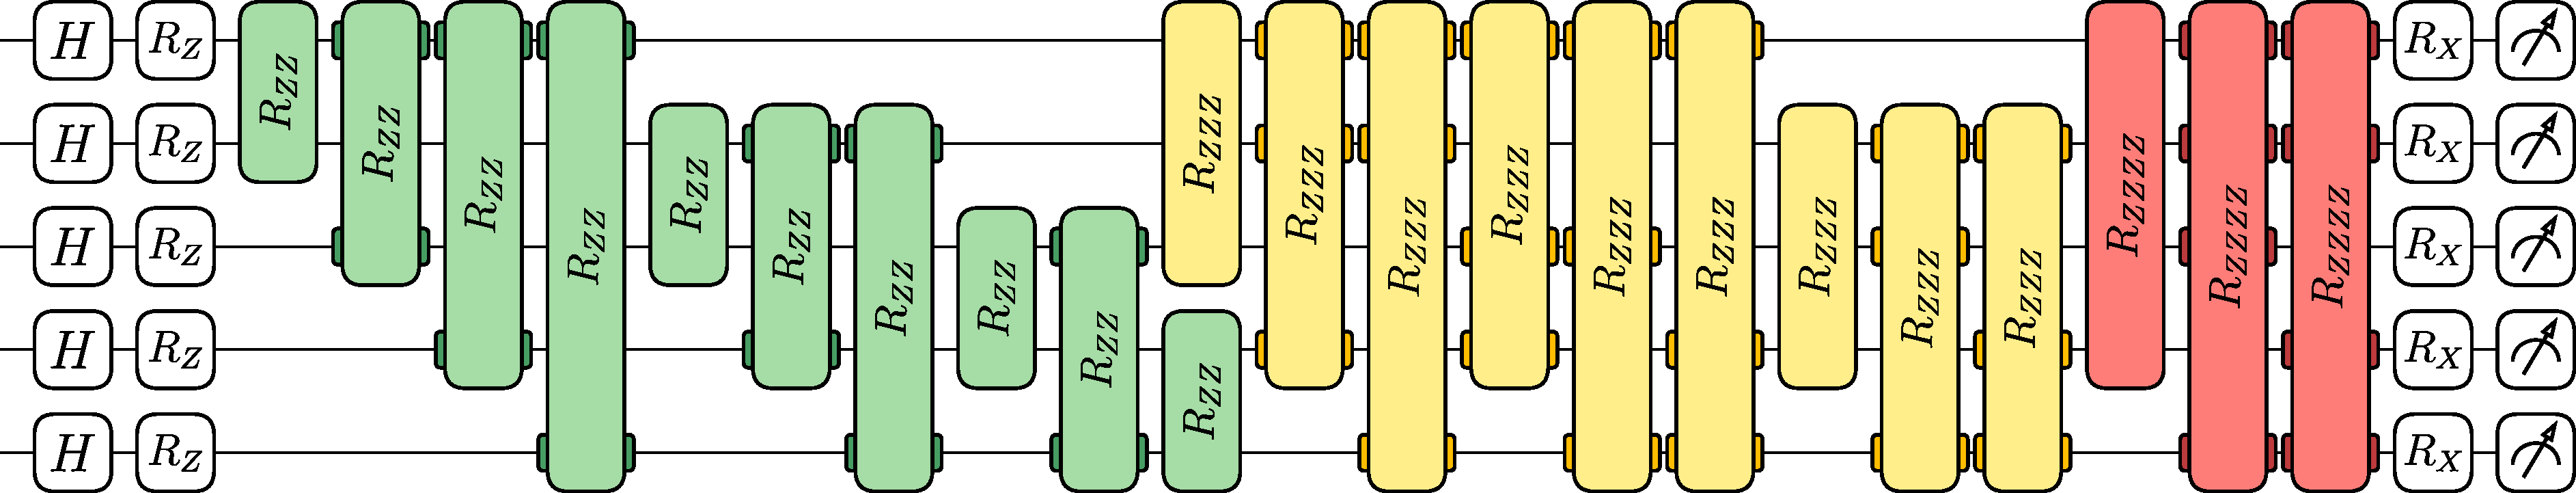
\includegraphics[width=1\textwidth]{02-factorization/figs/standard_circuit_35.pdf}
    \caption{One-layer circuit for factorizing the number $N=35$ using the standard QAOA protocol. Notice the presence
    of three- and four-qubit gates, highlighted in yellow and red, respectively. Rotation angles are omitted for simplicity.}
    \label{fig:standard_circuit}
\end{figure}

{\color{red} (FELIP: I found these few articles on QAOA factorization. The problem is that
they use simplification techniques and ad-hoc analysis to run factorization using much less qubits. I 
was not able to find articles that use the standard basic approach.)}

In a study that makes use of a similar approach, plus further pre-processing and simplifications, Anschuetz et al.
factorize numbers up to $291311$. Using additional classical pre-processing heuristics, Karamlou et al. were able to factorize
$1099551473989$, $3127$, and $6557$ using only $3$, $4$, and $5$ qubits, respectively. However, our aim is not to
compete with those approaches, since we focus on the general standard approach for factorization, without making use
of ad-hoc analysis.

\subsection{Our proposal (Linearized Protocol)}
As mentioned in the introduction to Section~\ref{Section:AFA}, the adiabatic factorization algorithm
needs to deal with the difficulty of implementing three- and four-body interaction terms. In the 
digitized version of this problem, like QAOA, this difficulty is transformed into three- and
four-qubit gates (Fig.~\ref{fig:standard_circuit}),
which need to be decomposed into multiple two-qubit gates (Fig.~\ref{fig:gate_decomposition}),
leading to lower fidelities at the end of the quantum circuit.

\begin{figure}[h]
    \centering
    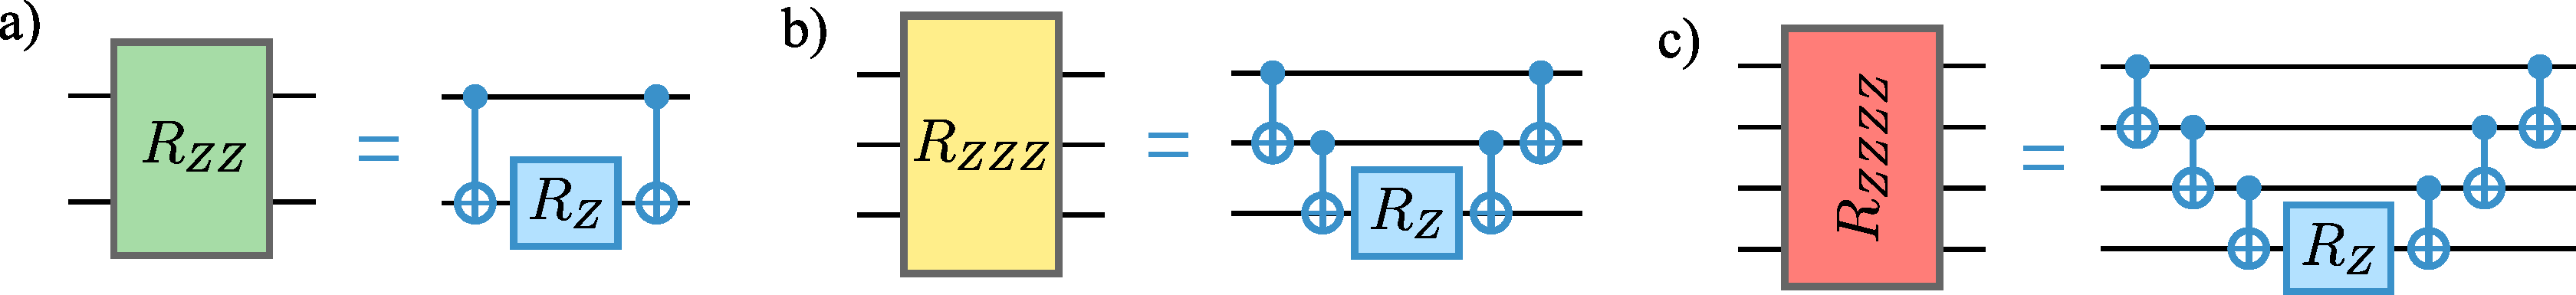
\includegraphics[width=1\textwidth]{02-factorization/figs/gate_decomposition.pdf}
    \caption{Decomposition of (a) two-, (b) three-, and (c) four-qubit Z-rotation gates in CNOTs and
    single-qubit Z-rotations.}
    \label{fig:gate_decomposition}
\end{figure}

To mitigate this issue, we propose a linearized problem Hamiltonian inspired by the same factorization condition, defined as:
\begin{equation}
	\hat{H}_\mathrm{LP} = N \1 - \bigg( \sum_{\ell=1}^{n_p} 2^\ell \hat{x}_\ell + \1 \bigg)
	\bigg( \sum_{m=1}^{n_q} 2^m \hat{y}_m + \1 \bigg)\,.
	\label{eq:linear_problem_hamiltonian}
\end{equation}
Unlike the original Hamiltonian $\hat{H}_\mathrm{QP}$, whose ground state encodes the solution, $\hat{H}_\mathrm{LP}$ contains only two-body terms and is therefore easier to implement, but the factorization solution corresponds to an eigenstate with eigenvalue zero rather than the ground state. Since the adiabatic theorem is not restricted to ground states but applies to any non-degenerate eigenstate, we hypothesize that it is possible to target this eigenstate through a suitable adiabatic or variational process. Based on this idea, our proposal is to replace the original Hamiltonian in the QAOA layers with $\hat{H}_\mathrm{LP}$, leveraging the possibility of starting from an eigenstate near the middle of the initial Hamiltonian’s spectrum and evolving under $\hat{H}_\mathrm{LP}$ to preserve this eigenstate structure, ultimately reaching the correct factorization solution, which also lies near the center of the spectrum.

\begin{figure}[h]
    \centering
    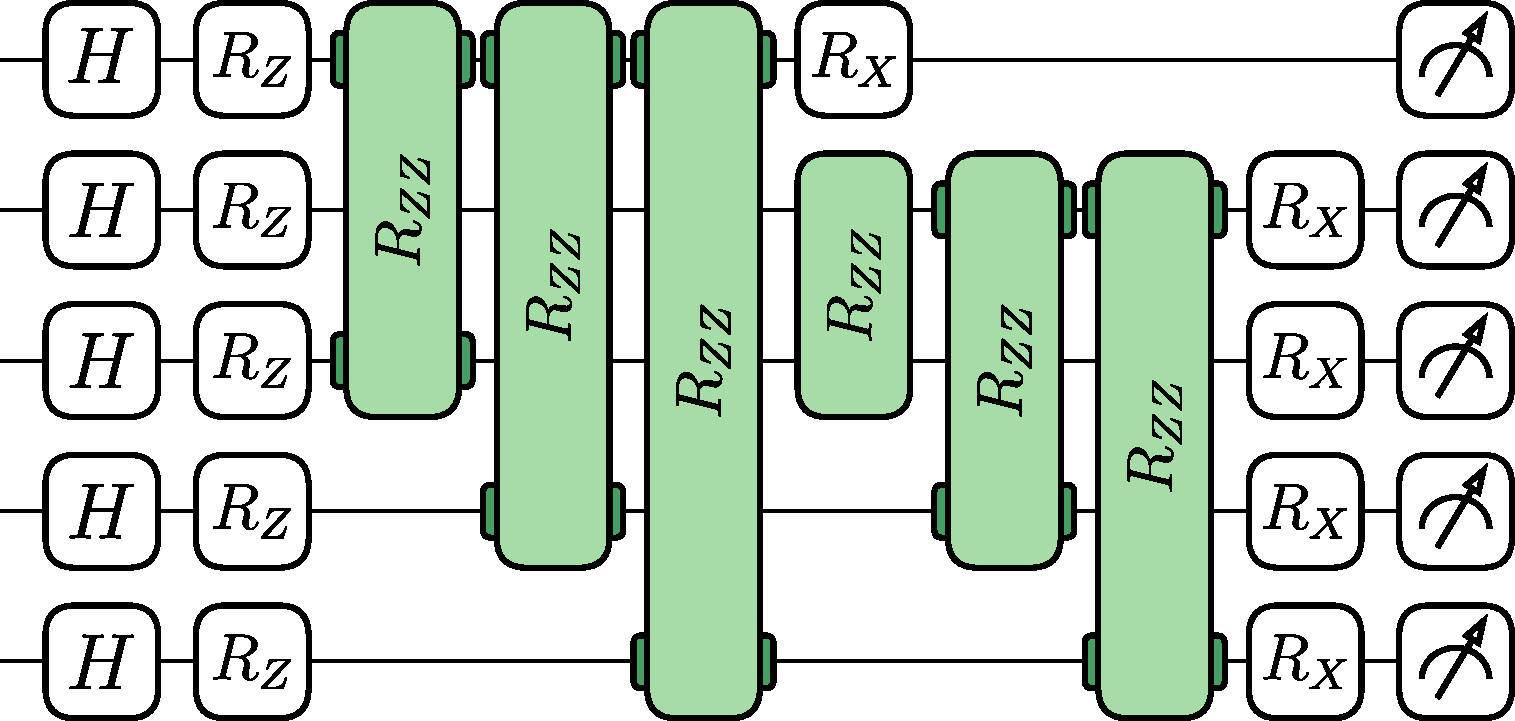
\includegraphics[width=0.55\textwidth]{02-factorization/figs/linear_circuit_35.pdf}
    \caption{One-layer circuit for factorizing the number $N=35$ using our protocol, evolving the state with the linear Hamiltonian $H_{\mathrm{LP}}$. Notice the simplification with respect to Fig.~\ref{fig:standard_circuit}
    due to the absence of three- and four-qubit gates.}
    \label{fig:linear_circuit_35.pdf}
\end{figure}

{\color{blue} (I am not sure if adding this paragraph or not, since at the end the cost function is just
a classical computation and maybe this explanation adds confusion.)}
There is another difference with respect to the standard QAOA protocol. In the latter, the same Hamiltonian
is typically used for both quantum state evolution and classical cost evaluation. In contrast,
our proposal explicitly decouples these two roles: we use the linearized Hamiltonian to drive the quantum
dynamics (problem Hamiltonian), and a separate cost Hamiltonian, whose ground state encodes the correct factors
to steer the classical optimizer.


%%%%%%%%%%%%%%%%%%%%%%%%%%%%%%%%%%%
% Chapter 3
%%%%%%%%%%%%%%%%%%%%%%%%%%%%%%%%%%%
\chapter{Results (work in progress)}
\label{Chapter:Results}

\dropcap{T}his chapter we introduce our results!!! To this end, we already can state here the problem of the many-body terms presented in the previous section. Then, we can be more clear in the next section.

\section{Benchmarking process}
To ensure a fair comparison between our proposed protocol and the standard QAOA approach, it is necessary to establish
consistent guidelines for the classical optimization process. For benchmarking, we adopt the configuration that yields
the best performance for the standard protocol. Specifically,
\begin{itemize}
    \item We employ the BFGS algorithm as the classical optimizer, which resulted in better performance
    than other optimizers such as L-BFGS-B (Fig.~\ref{fig:optimizer_comparison}) or Cobyla. Nelder-Mead has been discarded
    due to its poor scalability with the number of parametes.
    \item The QAOA parameters are trained using an incremental (layer-by-layer) approach: optimization begins with
    a single QAOA layer, and the optimal parameters obtained at each step are used to initialize the training of
    the next layer. {\color{red} (ADD REFERENCES)}
    \item In this initialization strategy, the parameters from the previous iteration are reused for the corresponding
    layers of the deeper circuit, while the new layer is initialized with its $\gamma$ parameter set equal to the last
    optimized $\gamma$ value and its $\beta$ parameter set to zero. This procedure improves convergence and reduces the
    likelihood of the optimizer becoming trapped in poor local minima, thereby providing a consistent reference
    for evaluating the performance of our protocol. {\color{red} (ADD REFERENCES)}
\end{itemize}
\section{Choosing a classical optimizer}
Many classical optimizers have been used within QAOA in literature \cite{blekos_review_2024}. However, we restricted ourselves
to some optimizers that are generally available in the very well-known SciPy Python's library, and tried different types: bounded,
unbounded, gradient-free, and gradient-based. For example, Nelder-Mead showed good performance, but it was discarded due to its bad
scalability with the number of parameters. Cobyla resulted in poor performance due to local minima trapping even for a few-qubit
problems, so it was also discarded. BFGS and L-BFGS-B are two gradient-based optimizers that were found to give the best results:
\begin{itemize}
    \item L-BFGS-B is a bounded optimizer that fits perfectly for QUBO and MaxCut problems. These problems contain symmetries
    that allow us to restrict the variational parameters into specific intervals, and this is the reason why it makes perfect
    sense to use a bounded optimizer in this cases.
    \item BFGS is an unbounded optimizer, i.e. the variational parameters can take any real value. We observed that this method
    outperforms L-BFGS-B in all the tested cases, up to 8--qubit problems. Our feeling is that BFGS is able to avoid some local
    minima in which L-BFGS-B gets trapped thanks to its unbounded nature.
\end{itemize}

\begin{figure}[h]
    \centering
    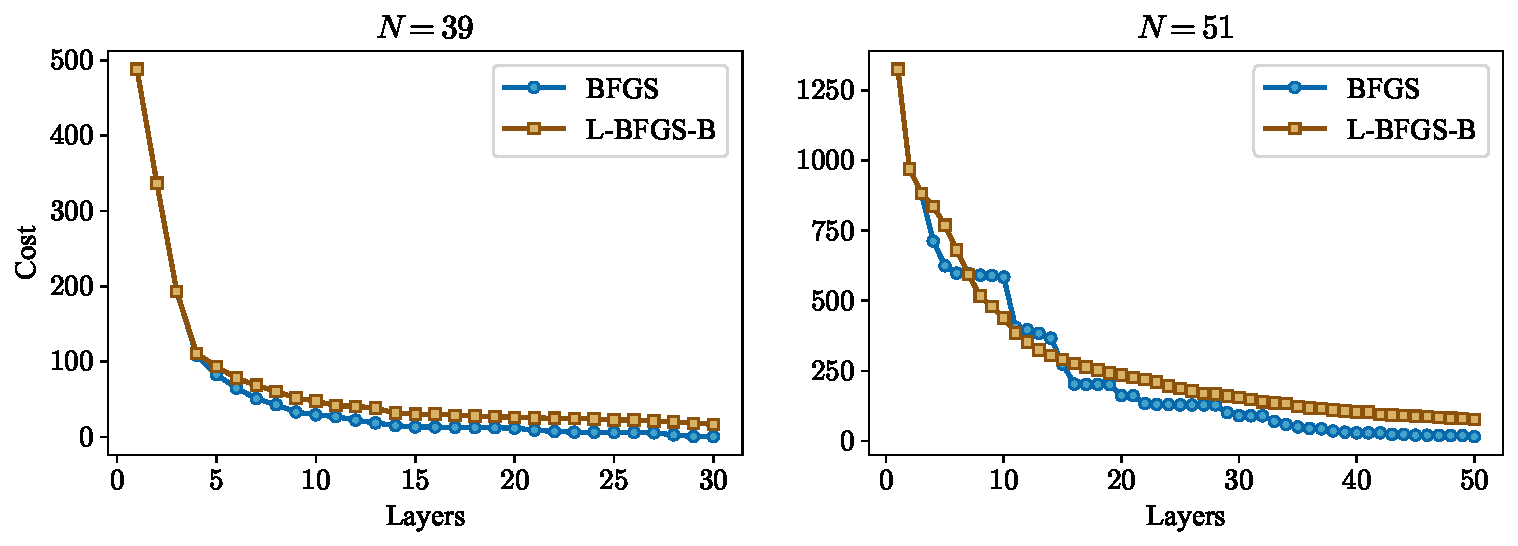
\includegraphics[width=1\textwidth]{03-results/figs/optimizer_comparison.pdf}
    \caption{Cost evolution comparison between BFGS and L-BFGS-B optimizers for factorizing $N=39$ and $N=51$
    using the standard protocol. These problems use 5 and 6 qubits, respectively, but the tendency has been observed
    up to 8-qubit problems.}
    \label{fig:optimizer_comparison}
\end{figure}

Many studies {\color{red} (add references, \cite{zhou_quantum_2020,diez-valle_universal_2025})} show how adiabatic-like passages surge in the
evolution of parameters through the different layers, where typically $\gamma$ --related to interaction field-- tends to start near
zero and increase monotonically until reaching a maximum value, while $\beta$ --related to transversal field-- starts at a maximum
value and decreases monotonically to zero. As shown in Fig.~\ref{fig:optimizer_parameter_comparison}, this behavior arises when
restricting variational parameters within specific intervals.

\begin{figure}[h]
    \centering
    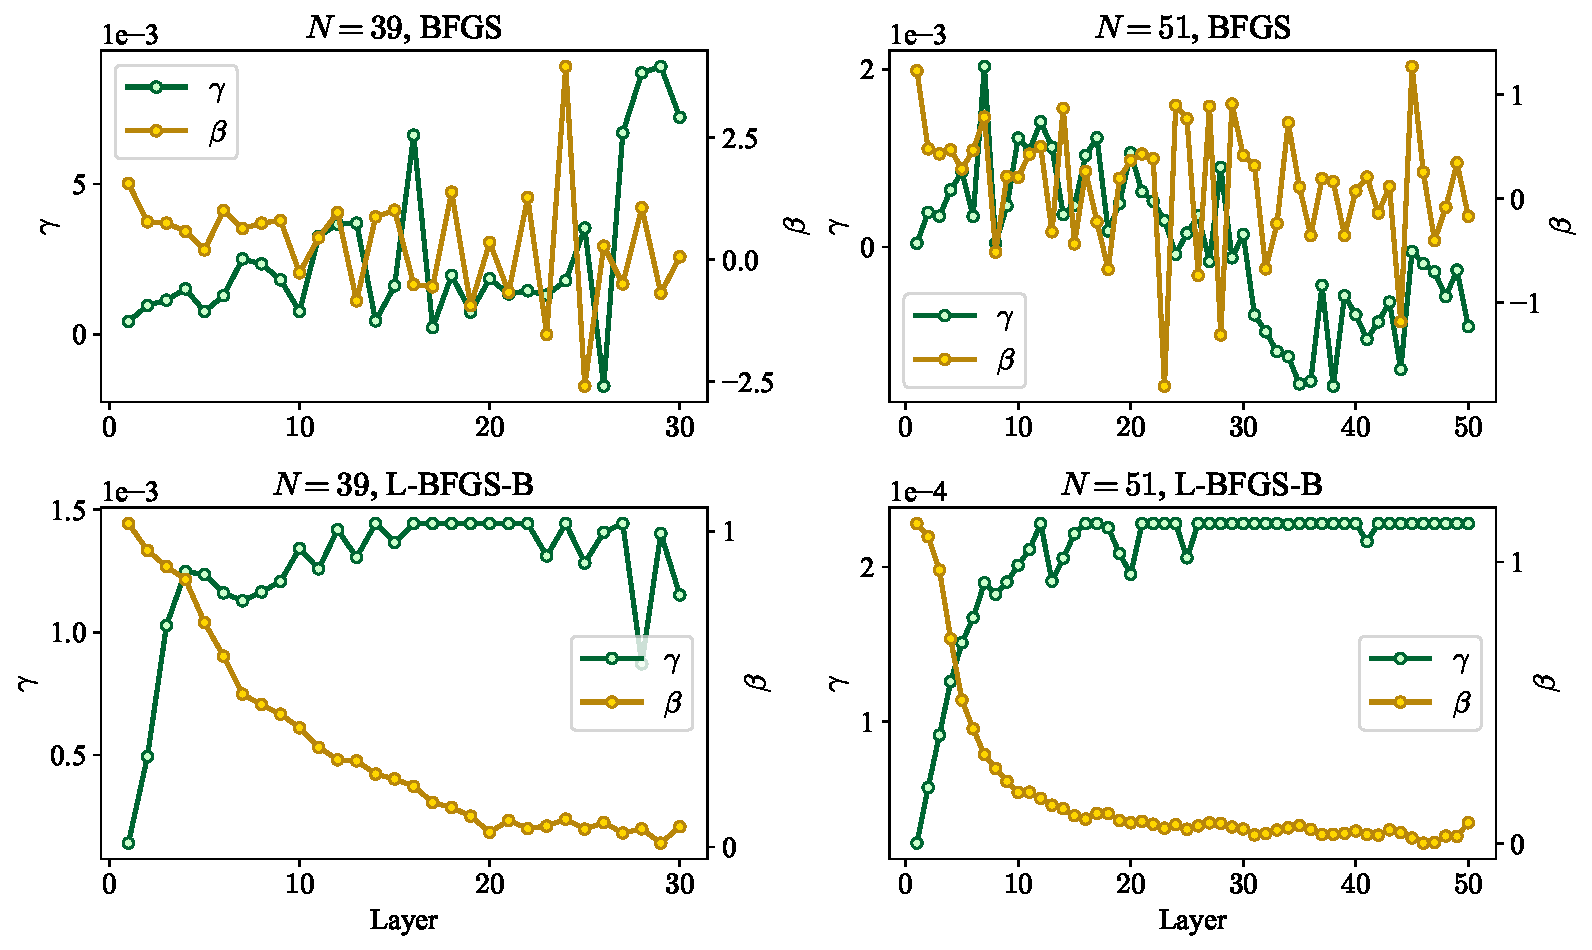
\includegraphics[width=1\textwidth]{03-results/figs/optimizer_parameters_comparison.pdf}
    \caption{Evolution of variational parameters for $N=39$ and $N=51$, using BFGS and L-BFGS-B classical optimizers for
    the standard protocol. Notice the adiabatic-like behavior of $\gamma$ and $\beta$ when using L-BFGS-B.}
    \label{fig:optimizer_parameter_comparison}
\end{figure}
\section{Results}
\lipsum[0-1]

\chapter{Conclusion}
\label{conclusion}

The conclusions of your thesis.


\section{This is a section title}

Hello have a table.

\begin{table}[t]
	\caption{A nice table.}
	\begin{tabular}{|l|l|}
		\hline
		Column name         & Explanation \\ \hline
		last\_modified      & Kaas        \\ \hline
		version             & Baas        \\ \hline
		db\_schema\_version & Haas        \\ \hline
	\end{tabular}
\end{table}

What? A booktabs table?

% Please add the following required packages to your document preamble:
% \usepackage{booktabs}
\begin{table}[t]
	\caption{A nice table.}
	\begin{tabular}{@{}ll@{}}
		\toprule
		Column name         & Explanation \\ \midrule
		last\_modified      & Kaas        \\
		version             & Baas        \\
		db\_schema\_version & Haas        \\ \bottomrule
	\end{tabular}
\end{table}

\subsection{This is a subsection}

Hi again!

\subsubsection{This is a subsubsection header}

Bye this time.


%%%%%%%%%%%%%%%%%%%%%%%%%%%%%%%%%%%
% CHAPTERS END
%%%%%%%%%%%%%%%%%%%%%%%%%%%%%%%%%%%





%% Use letters for the chapter numbers of the appendices.
%\appendix

%\include{appendix-a/appendix-a}

%% Turn off thumb indices for unnumbered chapters.
\thumbfalse



%%%%
% References
%%%%
\chapter*{Bibliography}
\addcontentsline{toc}{chapter}{Bibliography}
\setheader{Bibliography}


\bibliographystyle{unsrt}
% argument is your BibTeX string definitions and bibliography database(s)
\bibliography{bibliography}


%%%%
% Glossary
%%%%
\glsaddall
\printglossary[type=\acronymtype,title={Glossary}]
\addcontentsline{toc}{chapter}{Glossary}
\setheader{Glossary}



%%%%
% Thesis publications
%%%%
\chapter*{List of Publications}
\addcontentsline{toc}{chapter}{List of Publications}
\setheader{List of Publications}
\label{publications}

%% We use the 'etaremune' environment (the reverse of 'enumerate') to get a
%% numbered list of publications in reverse chronological order. If the list of
%% authors is long, it might be useful to emphasize your own name with \textbf.
\begin{etaremune}{\small
\item[\faFileTextO~~1.] \emph{Moritz Beller}: Toward an Empirical Theory of
  Feedback-Driven Development. To appear in 40th International Conference on
  Software Engineering (ICSE), Student Research Competition (SRC),
  Gothenborg, Sweden, 2018. Acceptance Rate 43\% (10/23)
}\end{etaremune}

\vspace{0.5cm}
\noindent
\faFileTextO~~Included in this thesis.\\
\faTrophy~~Won a best paper, tool demonstration, or proposal award.





\end{document}

